% Created 2016-08-25 jue 14:09
\documentclass[11pt]{article}
\usepackage[utf8]{inputenc}
\usepackage[T1]{fontenc}
\usepackage{fixltx2e}
\usepackage{graphicx}
\usepackage{grffile}
\usepackage{longtable}
\usepackage{wrapfig}
\usepackage{rotating}
\usepackage[normalem]{ulem}
\usepackage{amsmath}
\usepackage{textcomp}
\usepackage{amssymb}
\usepackage{capt-of}
\usepackage{hyperref}
\author{Claudio Vaucheret / Marcelo Amaolo}
\date{\textit{<2016-08-16 mar>}}
\title{Conceptos Avanzados en Lenguajes de Programación}
\hypersetup{
 pdfauthor={Claudio Vaucheret / Marcelo Amaolo},
 pdftitle={Conceptos Avanzados en Lenguajes de Programación},
 pdfkeywords={},
 pdfsubject={},
 pdfcreator={Emacs 24.4.1 (Org mode 8.3.2)}, 
 pdflang={English}}
\begin{document}

\maketitle
\tableofcontents


\section*{Introducción}
\label{sec:orgheadline29}

\subsection*{Razones para estudiar Conceptos de Lenguajes de Programación}
\label{sec:orgheadline1}
\begin{itemize}
\item Incrementa la habilidad para expresar ideas
\item Mejora la capacidad de elegir el lenguaje apropiado
\item Incrementa la capacidad de aprender nuevos lenguajes
\item Mejora el entendimiento del funcionamiento interno del lenguaje
(implementación)
\end{itemize}

\subsection*{Dominios de Programación}
\label{sec:orgheadline2}
\begin{itemize}
\item Aplicaciones Científicas
\begin{itemize}
\item Gran número de computación de punto flotante
\item Fortran
\end{itemize}
\item Aplicaciones Empresariales
\begin{itemize}
\item Producción de Reportes, uso de números decimales y caracteres
\item Cobol
\end{itemize}
\item Inteligencia Artificial
\begin{itemize}
\item Manipulación simbólica (en lugar de números)
\item LISP
\end{itemize}
\item Sistemas de Programación
\begin{itemize}
\item Necesidad de eficiencia (debido al uso continuo)
\item C
\end{itemize}
\item Software para la WEB
\begin{itemize}
\item Colección ecléctica de lenguajes: maukup (e.g. HTML5), scripting
(e.g. PHP), de propósito general (e.g. Java)
\end{itemize}
\end{itemize}

\subsection*{Criterios de Evaluación de Lenguajes}
\label{sec:orgheadline8}
\begin{itemize}
\item \textbf{Legibilidad}: la facilidad con la cual los programas pueden ser
leídos y entendidos.
\item \textbf{Escribilidad}: la facilidad con la cual un lenguaje puede ser usado
para crear programas
\item \textbf{Confiabilidad}: El grado en que el lenguaje funciona de acuerdo a
sus especificaciones.
\item \textbf{Costo}: de uso, compilación, mantenimiento etc.
\end{itemize}

\subsubsection*{Legibilidad}
\label{sec:orgheadline3}
\begin{itemize}
\item Simplicidad
\begin{itemize}
\item Un conjunto manejable de características y construcciones
\item Poca multiplicidad de características (medios de realizar la misma operación)
\item Minima sobrecarga de operadores
\end{itemize}
\item Ortogonalidad
\begin{itemize}
\item Un conjunto relativamente pequeño de construcciones primitivas que
puedan ser combinadas en un numero pequeño de modos
\item Toda posible combinación sea legal.
\end{itemize}
\item Sentencas de Control
\begin{itemize}
\item La presencia de bien conocidas estructuras de control
\end{itemize}
\item Tipos de Datos y Estructuras
\begin{itemize}
\item La presencia de facilidades adecuadas para definir estructuras de datos
\end{itemize}
\item Consideraciones sintácticas
\begin{itemize}
\item Composición flexible de identificadores
\item Palabras especiales y métodos para formar sentencias compuestas
\item Construcciones autodescriptivas, palabras reservadas
significativas
\end{itemize}
\end{itemize}

\subsubsection*{Escribilidad}
\label{sec:orgheadline4}

\begin{itemize}
\item Simplicidad y ortogonalidad
\begin{itemize}
\item Pocas constucciones, numero pequeño de primitivas y pocas reglas
para combinarlas.
\end{itemize}
\item Soporte para la abstracción
\begin{itemize}
\item La habilidad para definir y usar estructuras complejas u
operaciones de modo que los detalles puedan ser ignorados
\end{itemize}
\item Expresibilidad
\begin{itemize}
\item Un conjunto conveniente de modos de especificar operaciones
\item Ejemplo: La inclusión de la sentencia \textbf{FOR} en  muchos lenguajes modernos
\end{itemize}
\end{itemize}

\subsubsection*{Confiabilidad}
\label{sec:orgheadline5}

\begin{itemize}
\item Chequeo de Tipos
\begin{itemize}
\item verificación de errores de tipos
\end{itemize}
\item Manejo de Excepciones
\begin{itemize}
\item interceptar errores en ejecución y tomar medidas correctivas
\end{itemize}
\item Aliasing
\begin{itemize}
\item Presencia de dos o mas distintas referencias para el mismo lugar
de memoria
\end{itemize}
\item Legibilidad y Escribilidad
\begin{itemize}
\item Un lenguage que no soporta modos "naturales" de expresar un
algoritmo necesariamente usará aproximaciones "no naturales" y asi
reducirá la confiabilidad
\end{itemize}
\end{itemize}

\subsubsection*{Costo}
\label{sec:orgheadline6}
\begin{itemize}
\item Costo de \ldots{}
\begin{itemize}
\item Entrenar programadores para usar un lenguaje
\item Escribir programas (cercano a aplicaciones particulares)
\item Compilar programas
\item Ejecutar programas
\item Implementar Lenguajes (disponibilidad de compiladores libres)
\item Confiabilidad: Confiabilidad pobre lleva a altos costos
\item Mantener programas
\end{itemize}
\end{itemize}

\subsubsection*{Otros}
\label{sec:orgheadline7}
\begin{itemize}
\item Portabildad
\begin{itemize}
\item La facilidad con que los programas puedan moverse de una
implementación a otra
\end{itemize}
\item Generalidad
\begin{itemize}
\item Su aplicabilidad a un amplio rango de aplicaciones.
\end{itemize}
\item Bien definido
\begin{itemize}
\item La completitud y precisión de la definición oficial del lenguaje
\end{itemize}
\end{itemize}

\subsection*{Influencias en el diseño de los lenguajes}
\label{sec:orgheadline14}
\begin{itemize}
\item Arquitectura de Computadoras
\begin{itemize}
\item Lenguajes son desarrollados alrededor de la arquitectura de
computadora prevaleciente, conocida como arquitectura de \emph{von Neumann}
\end{itemize}
\item Metodologías de Programación
\begin{itemize}
\item Nuevas metodologías de desarrollo de software (e.g. desarrollode
software orientado a objetos) llevan a nuevos paradigmas y por
extensión a nuevos lenguajes de programación
\end{itemize}
\end{itemize}

\subsubsection*{Influencia de la Arquitectura de Computadoras}
\label{sec:orgheadline9}

\begin{itemize}
\item Arquitectura de Computadora bien conocida: Von Neumann
\item Lenguajes Imperativos mas dominantes debido a la arquitectura
dominante
\begin{itemize}
\item Datos y Programas almacenados en memoria
\item Memoria Separada de la CPU
\item Instrucciones y Datos son conducidos desde la Memoria a la CPU
\item Bases para los lenguajes imperativos
\begin{itemize}
\item Variables modelan celdas de memoria
\item La iteración es eficiente
\end{itemize}
\end{itemize}
\end{itemize}

\subsubsection*{Arquitectura de Von Neumann}
\label{sec:orgheadline10}

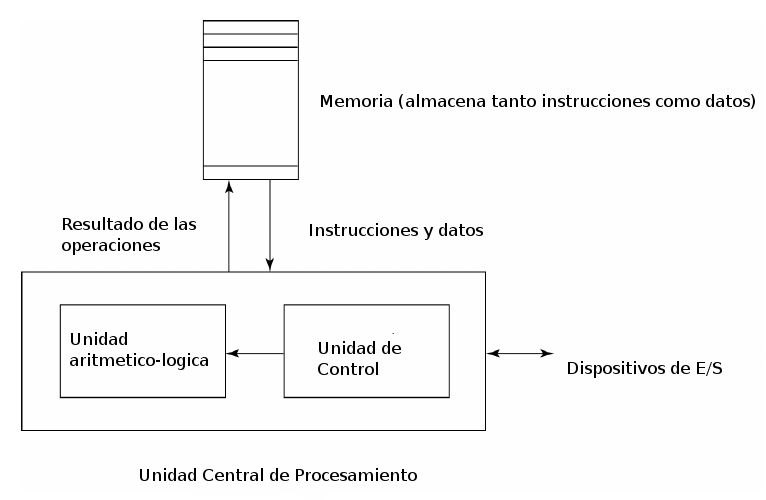
\includegraphics[width=.9\linewidth]{vonneumann.png} 

\subsubsection*{Influencia de las Metodogías de Programación}
\label{sec:orgheadline11}
\begin{itemize}
\item Décadas de los 50 y 60: Simples aplicaciones; preocupación principal
la eficiencia
\item Finales de los 60: Eficiencia de programación toma importancia:
legibilidad, mejores estructuras de control
\begin{itemize}
\item Programación Estructurada
\item Diseño \emph{top-down} y refinamiento \emph{step-wise}
\end{itemize}
\item Finales de los 70: De Orientación a Procesos a Orientación a Datos.
\begin{itemize}
\item Abstracción de Datos
\end{itemize}
\item Mediados de los 80: Programación orientada a Objetos
\begin{itemize}
\item Abstracción de Datos + Herencia + Polimorfismo
\end{itemize}
\end{itemize}

\subsubsection*{Categoría de Lenguajes}
\label{sec:orgheadline12}
\begin{itemize}
\item Imperativa
\begin{itemize}
\item Variables, sentencias de asignación e iteración
\item Ejemplos: C, Pascal
\end{itemize}
\item Funcional
\begin{itemize}
\item Principal medio de computación es aplicar funciones a parámetros
\item Ejemplos: LISP, Scheme
\end{itemize}
\item Lógica
\begin{itemize}
\item Basado en Reglas
\item Ejemplo: Prolog
\end{itemize}
\item Orientado a Objetos
\begin{itemize}
\item abstracción de datos, herencia, ligadura tardía
\item Ejemplos: Java, C++
\end{itemize}
\item Marcado
\begin{itemize}
\item No programación per se, pero usados para especificar la
información mostrada en documentos web
\item Ejemplos: XHTML, XML
\end{itemize}
\end{itemize}

\subsubsection*{Compromisos en el diseño de Lenguajes}
\label{sec:orgheadline13}
\begin{itemize}
\item Confiabilidad vs. Costo de ejecución
\begin{itemize}
\item Ejemplo: Java exige que todas las referencias a elementos de los
arreglos sean chequeadas si la indexación es correcta, pero esto
incrementa el costo de ejecución
\end{itemize}
\item Legibilidad vs. Escribilidad
\begin{itemize}
\item Ejemplo: APL provee muchos operadores poderosos (y un gran numero
de nuevos simbolos) permitiendo que complejas operaciones sean
escritas en un programa compacto pero con el costo de pobre legibilidad
\end{itemize}
\item Flexibilidad vs. Confiabilidad
\begin{itemize}
\item Ejemplo: Los punteros de C++ son poderosos y muy flexibles pero de
un uso poco confiable.
\end{itemize}
\end{itemize}

\subsection*{Métodos de Implementación}
\label{sec:orgheadline28}
\begin{itemize}
\item Compilación
\begin{itemize}
\item Los programas son traducidos al lenguaje máquina
\end{itemize}
\item Interpretación Pura
\begin{itemize}
\item Los programas son interpretados por otro programa llamado intérprete
\end{itemize}
\item Sistemas de implementación híbridos
\begin{itemize}
\item Un compromiso entre compilación y interpretación pura
\end{itemize}
\end{itemize}

\subsubsection*{Capas de Implementación de Lenguajes}
\label{sec:orgheadline15}

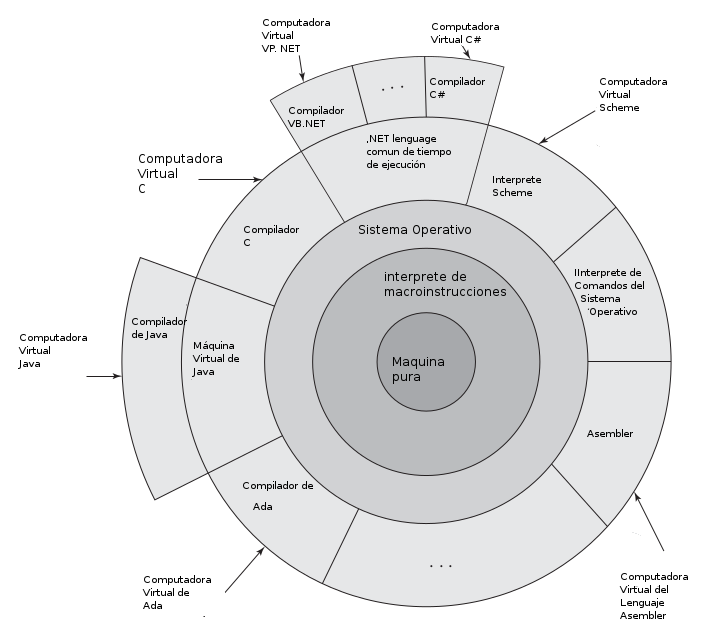
\includegraphics[width=.9\linewidth]{interfacecapas.png}

\subsubsection*{Compilación}
\label{sec:orgheadline16}
\begin{itemize}
\item Traduce programas de alto nivel (lenguaje fuente) en codigo máquina
\item Traducción lenta, ejecución rápida
\item El proceso de compilación tiene varias faces:
\begin{itemize}
\item análisis lexico: convierte caracteres del programa fuente en
unidades léxicas
\item análisis sintáctico: Transforma unidades léxicas en árboles
sintácticos \emph{parse trees}
\item análisis semántico: Genera código intermedio
\item generación de código: Codigo máquina es generado
\end{itemize}
\end{itemize}

\subsubsection*{El proceso de compilación}
\label{sec:orgheadline17}

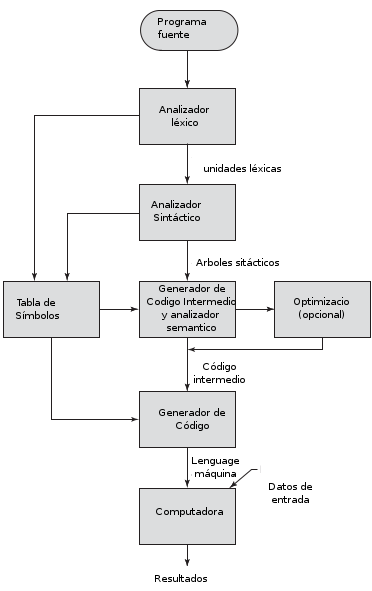
\includegraphics[width=.9\linewidth]{procesocomp.png} 

\subsubsection*{Terminología Adicional de Compilación}
\label{sec:orgheadline18}

\begin{itemize}
\item Módulo de carga (imagen ejecutable) : El código del usuario y del
sistema juntos
\item \emph{linking and loading} Enlazado y Carga: El proceso de recolectar los
programas del sistema y enlazarlo al programa del usuario
\end{itemize}

\subsubsection*{Ejecución del Código Máquina}
\label{sec:orgheadline19}

\begin{itemize}
\item ciclo de traer y ejecutar (sobre una arquitectura Von Neumann)
\end{itemize}

\begin{verbatim}
repeat  por siempre
   traer la instrucción apuntada por el contador
   incrementar el contador
   decodificar la instrucción
   ejecutar la instrucción
end repeat
\end{verbatim}

\subsubsection*{\emph{Cuello de botella} de Von Neumann}
\label{sec:orgheadline20}

\begin{itemize}
\item La velocidad de conección entre la memoria de la computadora y su
procesador determina la velocidad de la computadora
\item Las intrucciones del programa son ejecutadas mucho mas rápido que la
velocidad de conección; por lo tanto ésta se vuelve el \emph{cuello de botella}
\item Es conocido que \emph{cuello de botella} de la arquitectura de Von
Neumann es el principal factor en la velocidad de las computadoras
\end{itemize}

\subsubsection*{Interpretación Pura}
\label{sec:orgheadline21}
\begin{itemize}
\item Sin traducción
\item Facil implementación de programas. Errores de tiempo de ejecución
pueden ser facilmente reconocidos
\item Ejecución mas lenta (10 a 100 veces mas lenta que programas compilados)
\item Frecuentemente requiere mas espacio
\item Se volvio infrecuente en lenguajes de alto nivel
\item Han retornado con lenguajes de \emph{sripting} para la Web (e.g. JavaScript)
\end{itemize}

\subsubsection*{Proceso de Interpretación Pura}
\label{sec:orgheadline22}

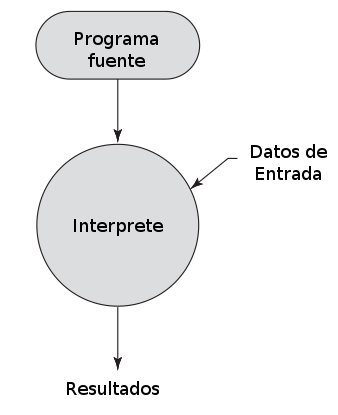
\includegraphics[width=.9\linewidth]{procesointerppuro.png}

\subsubsection*{Sistemas de Implementación Híbrida}
\label{sec:orgheadline23}
\begin{itemize}
\item Un compromiso entre compilador y intérprete puro
\item El programa en lenguaje de alto nivel es traducido a un lenguaje
intermedio que permite facil interpretación
\item Mucho mas rápido que interpretación pura
\item Ejemplos
\begin{itemize}
\item Programas en Perl son parcialmente compilados para detectar
errores antes de la interpretación
\item Implementaciones iniciales de Java fueron híbridas, la forma
intermedia \emph{byte code}, proveyó portabilidad a toda máquina que
tenía un interprete de \emph{byte code} y un sistema de \emph{run time}
(juntos son llamados la máquina virtual de java)
\end{itemize}
\end{itemize}

\subsubsection*{Proceso de Implementación Híbrida}
\label{sec:orgheadline24}

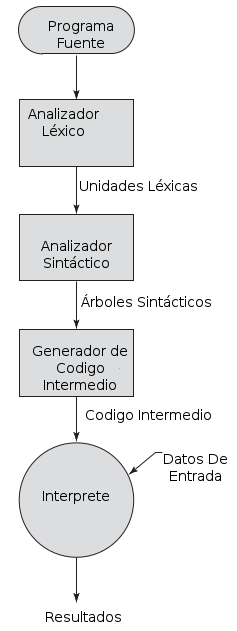
\includegraphics[width=.9\linewidth]{procesohibrido.png} 

\subsubsection*{Sistemas de Implementación \emph{Just in Time}}
\label{sec:orgheadline25}
\begin{itemize}
\item Inicialmente Los programas se traducen a un lenguaje intermedio
\item Luego el lenguaje intermedio se compila a código máquina
\item La versión en máquina se conserva para llamadas subsecuentes
\item Sistemas JIT son ampliamente usados para programas Java
\item Lenguajes .NET son implementados con sistemas JIT
\end{itemize}

\subsubsection*{Preprocesadores}
\label{sec:orgheadline26}
\begin{itemize}
\item Macros de preprocesamiento (instrucciones) son comunmente usadas
para especificar que código de otros archivos sean incluidos
\item Un preprocesador procesa un programa inmediatamente antes de que el
programa se compile para expandir las macros incluídas
\item Un ejemplo conocido: El preprocesador de C
\begin{itemize}
\item expands \#include, \#define, y macros similares
\end{itemize}
\end{itemize}

\subsubsection*{Entornos de Programación}
\label{sec:orgheadline27}
\begin{itemize}
\item Una colección de herramientas usadas en el desarrollo de software
\item UNIX
\begin{itemize}
\item un tradicional sistema operativo y colección de herramientas
\item hoy en dia frecuentemente usado a través de un GUI que corren
sobre UNIX
\end{itemize}
\item Borland JBuilder
\begin{itemize}
\item Un entorno de programación integrado para Java
\end{itemize}
\item Microsoft Visual Studio .NET
\begin{itemize}
\item Un complejo entorno visual de desarrollo
\item Usado para programar en C\#, Visual Basic .NET, jscript, J\# o C++
\end{itemize}
\end{itemize}


\section*{Evolución de los Lenguajes de Programación}
\label{sec:orgheadline103}

\subsection*{Lenguajes de Programación}
\label{sec:orgheadline30}

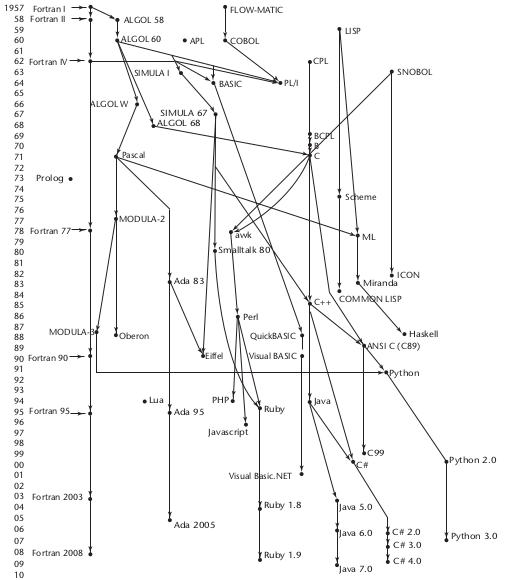
\includegraphics[width=.9\linewidth]{evolleng.png}

\subsection*{Evolución de los primeros lenguajes}
\label{sec:orgheadline31}

\subsection*{Konrad Zuze's language de la computadora Z4.}
\label{sec:orgheadline33}

\subsubsection*{Zuse's Plankalkül}
\label{sec:orgheadline32}

\begin{itemize}
\item Desarrollado en 1945
\item Nunca implementado
\item Su descripción fue publicada en 1972.
\item Tipos de datos: bit, Integer and float tipos compuestos.
\item arreglos y registros
\end{itemize}

\begin{verbatim}
  | A + 1 => A
V | 4        5
S | 1.n      1.n
\end{verbatim}




\subsection*{Codigo Máquina: pseudocodigos ¿?}
\label{sec:orgheadline38}

\subsubsection*{Escribir en lenguaje máquina}
\label{sec:orgheadline34}

\begin{itemize}
\item poco legibles y modificables
\item sin indices ni punto flotante
\item direccionamiento absoluto
\end{itemize}

\subsubsection*{Shorte Code Mauchly (1949)}
\label{sec:orgheadline35}

\begin{itemize}
\item computadora BINAC
\item Expresiones eran codificadas de izquierda a derecha
\item Ejemplos de operaciones:
\end{itemize}

\begin{verbatim}
01 - 06 abs value 1n (n+2)nd power
02 ) 07 +         2n (n+2)nd root
03 = 08 pause     4n if <= n
04 / 09 (         58 print and tab
\end{verbatim}

La sentencia X0 = SQRT(ABS(Y0)) podria ser codificada como:

\begin{verbatim}
00 X0 03 20 06 Y0
\end{verbatim}

\subsubsection*{Speedcoding}
\label{sec:orgheadline36}

\begin{itemize}
\item Desarrollado por John Backus en 1954 para IBM 701
\item Pseudo operaciones para funciones aritméticas y matemtaticas
\begin{itemize}
\item bifurcación condicional e incondicional
\item registros autoincrementales para acceso a arreglos
\item 4.2 millisegundos la instruccion de suma y 700 palabras para el programa
\item 2 semanas de programación en pocas horas!!!
\end{itemize}
\end{itemize}

\subsubsection*{Otros sistemas relacionados}
\label{sec:orgheadline37}

\begin{itemize}
\item Sistema de "compilación" UNIVAC
\begin{itemize}
\item Desarrollado por el equipo de Brace Hopper
\item Pseudocodigo expandido en código máquina (macros)
\end{itemize}
\item David J Wheeler (Universidad de Cambridge) (1950)
\begin{itemize}
\item Desarrollo un método de usar bloques de direccionamiento reubicables
\end{itemize}
\item Wilkes (1951-1957) desarrollo lenguaje \emph{assembler} con estas ideas
\end{itemize}


\subsection*{IBM 704 y Fortran}
\label{sec:orgheadline48}

\subsubsection*{Fortan}
\label{sec:orgheadline39}
\begin{itemize}
\item Fortran 0: 1954 - no implementado
\item Fortran 1 1957
\begin{itemize}
\item Diseñado para la nueva IBM 704, que tenía registros y aritmética
de punto flotante
\item Entorno de Desarrollo
\begin{itemize}
\item Las Computadoras eran pequeñas y confiables
\item Las aplicaciones eran científicas
\item Sin metodología ni herramientas de programación
\item Importancia en \textbf{eficiencia}
\end{itemize}
\end{itemize}
\end{itemize}

\subsubsection*{Proceso de Diseño}
\label{sec:orgheadline40}
\begin{itemize}
\item El impacto del entorno en el diseño de Fortran
\begin{itemize}
\item Sin necesidad de almacenamiento dinámico
\item Necesidad de un buen manejo de arreglos y ciclos
\item Sin manejo de cadenas, aritmética decimal o herramientas de
entrada/salida (de uso comercial)
\end{itemize}
\end{itemize}

\subsubsection*{Fortran I}
\label{sec:orgheadline41}
\begin{itemize}
\item Primera versión implementada de Fortrand
\begin{itemize}
\item Nombres hasta 6 caracteres
\item Ciclos iterativos con post condición (\textbf{DO})
\item I/O formateada
\item subprogramas definidos por el usuario
\item Sentencias condicionales de tres modos (\textbf{IF} aritmético)
\item sentencias sin tipo de datos
\end{itemize}
\end{itemize}

\subsubsection*{Fortran I}
\label{sec:orgheadline42}
\begin{itemize}
\item Primera versión implementada
\begin{itemize}
\item Sin compilación separada
\item Compilador distribuido en Abril de 1957,
\item Programas de mas de 400 lineas raramente compilaban correctamente,
principalmente debido a la pobre confiabilidad de la IBM 704
\item La Codificación era verdaderamente rápida
\item Rapidamente se volvió ampliamente usado
\end{itemize}
\end{itemize}

\subsubsection*{Fortran II}
\label{sec:orgheadline43}
\begin{itemize}
\item Distribuido en 1958
\begin{itemize}
\item Compilación independiente
\item Se corrigieron muchos errores
\end{itemize}
\end{itemize}

\subsubsection*{Fortran IV}
\label{sec:orgheadline44}
\begin{itemize}
\item Desarrollado durante 1960-1962
\begin{itemize}
\item Declaración explicita de tipos
\item Sentencia de selección lógica
\item Nombres de programas podian se pasados como parámetros
\item ANSI standard en 1966
\end{itemize}
\end{itemize}

\subsubsection*{Fortran 77}
\label{sec:orgheadline45}
\begin{itemize}
\item Se volvió el nuevo estandard en 1978
\begin{itemize}
\item Manejo de cadenas de caracteres
\item sentencia de control de ciclos lógico
\item sentencia \textbf{IF-THEN-ELSE}
\end{itemize}
\end{itemize}

\subsubsection*{Fortran 90}
\label{sec:orgheadline46}
\begin{itemize}
\item Con los mas significativos cámbios desde el Fortran 77
\begin{itemize}
\item Módulos
\item Arreglos dinámicos
\item Punteros
\item Recursión
\item sentencia \textbf{CASE}
\item chequeo de tipos en los parametros
\end{itemize}
\end{itemize}

\subsubsection*{Evaluación de Fortran}
\label{sec:orgheadline47}
\begin{itemize}
\item Compiladores altamente optimizados (todas las versiones anteriores a 90)
\begin{itemize}
\item Los tipos y almacenamiento de todas las variables eran fijas antes del
tiempo de ejecución.
\end{itemize}
\item Dramaticamente cambió para siempre el modo en que las computadoras
fueron usadas
\item Caracterizados como la \emph{lingua franca} del mundo de la computación
\end{itemize}


\subsection*{Programación Funcional: LISP}
\label{sec:orgheadline54}

\subsubsection*{LISP}
\label{sec:orgheadline49}
\begin{itemize}
\item \emph{LISt Processing Language}
\begin{itemize}
\item Diseñado en el MIT por McCarthy
\end{itemize}
\item Investigación en AI necesitaba un lenguaje
\begin{itemize}
\item Procesamiento de datos en Listas (en lugar de arreglos)
\item Computación simbólica (en lugar de numérica)
\end{itemize}
\item Solo dos tipos de datos: átomos y listas
\item Basado en el \textbf{Lambda calculus}
\end{itemize}

\subsubsection*{Representación de Listas LISP}
\label{sec:orgheadline50}

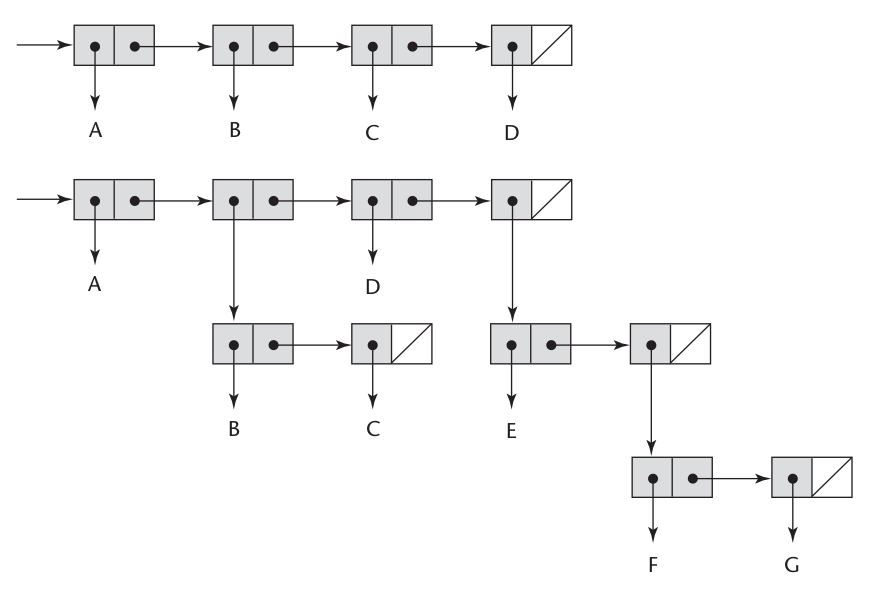
\includegraphics[width=.9\linewidth]{represlistas.png}

\subsubsection*{Evaluación de LISP}
\label{sec:orgheadline51}
\begin{itemize}
\item Pionero en programación funcional
\begin{itemize}
\item Sin necesidad de variables o asignación
\item Control via recursión y expresiones condicionales
\end{itemize}
\item Aún un lenguaje dominante para IA
\item COMMON LISP y Scheme son dialectos contemporaneos de LISP
\item ML, Miranda, Haskell son lenguajes relacionados
\end{itemize}

\subsubsection*{Scheme}
\label{sec:orgheadline52}
\begin{itemize}
\item Desarrollado en el MIT a mediados de los 70
\item Pequeño
\item Extensivo uso de alcance estático
\item Funciones como entidades de primera clase
\item Sintaxis simple, ideal para aplicaciones educativas
\end{itemize}

\subsubsection*{COMMON LISP}
\label{sec:orgheadline53}
\begin{itemize}
\item Un esfuerzo por combinar características de varios dialectos de LISP
en un solo lenguaje
\item Grande y Complejo
\end{itemize}

\subsection*{Primera sofisticación: ALGOL 60}
\label{sec:orgheadline62}

\subsubsection*{Algol 60}
\label{sec:orgheadline55}
\begin{itemize}
\item Entorno de Desarrollo
\begin{itemize}
\item FORTRAN había arribado para las IBM 70x
\item Muchos lenguajes se habían desarrollado para máquinas específicas
\item Ningún lenguaje era portable; todos eran dependiente de las máquinas
\item No existía ningún lenguaje universal para comunicar algoritmos
\end{itemize}
\item ALGOL 60 fue el resultado del esfuerzo de designar un lenguaje universal
\end{itemize}

\subsubsection*{Primitivo proceso de diseño}
\label{sec:orgheadline56}
\begin{itemize}
\item Encuentro de ACM y GAMM para cuatro dias de diseño (27 de Mayo al 1
de Junio de 1958)
\item Metas del Lenguaje
\begin{itemize}
\item Cercano a la notación matemática
\item Bueno para describir algoritmos
\item Traducible a lenguaje máquina
\end{itemize}
\end{itemize}

\subsubsection*{ALGOL 58}
\label{sec:orgheadline57}
\begin{itemize}
\item El concepto de tipos fue formalizado
\item Los nombre podrían tener cualquier longitud
\item Los arreglos podrían tener cualquier número de subíndices
\item Los parámetros fueron separados por modo (Entrada y Salida)
\item Subíndices fueron colocados entre corchetes
\item Sentencias compuestas (\textbf{begin \ldots{} end})
\item Punto y coma como separador de sentencias
\item Operador de asignación fue \textbf{:=}
\item \textbf{if} tenía una cláusula \textbf{else-if}
\item Sin E/S - "podría hacerlo dependiente de la máquina"
\end{itemize}

\subsubsection*{Implementación de ALGOL 58}
\label{sec:orgheadline58}
\begin{itemize}
\item Sin intención de ser implementado, sin embargo variaciones de él si
lo fueron (MAD, JOVIAL)
\item Aunque IBM fue inicialmente entusiasta, todo soporte fue quitado a
mediados de 1959
\end{itemize}

\subsubsection*{ALGOL 60}
\label{sec:orgheadline59}
\begin{itemize}
\item Se modificó ALGOL 58 en una reunión de 6 dias en Paris
\item Nuevas Características
\begin{itemize}
\item Estructura de bloques (alcance local)
\item Dos métodos de pasaje de parámetros
\item Recursión de subprogramas
\item arreglos dinámicos (basados en pilas)
\item Todavía sin E/S ni manejo de cadenas de caracteres
\end{itemize}
\end{itemize}

\subsubsection*{Evaluación de ALGOL 60}
\label{sec:orgheadline60}
\begin{itemize}
\item Exitoso
\begin{itemize}
\item Fue el modo estándar de publicar algoritmos por los siguientes 20 años
\item Todo subsecuente lenguaje imperativo fue basado en él
\item Primer lenguaje independiente de la máquina
\item Primer lenguaje cuya sintaxis fue formalmente definida (BNF)
\end{itemize}
\end{itemize}

\subsubsection*{Evaluación de ALGOL 60}
\label{sec:orgheadline61}
\begin{itemize}
\item Fracaso
\begin{itemize}
\item Nunca fue ampliamente usado, especialmente en U.S.
\item Razones:
\begin{itemize}
\item Falta de E/S y el conjunto de caracteres lo hacía no portable
\item Demasiado flexible para implementar
\item atrincheramiento de Fortran
\item Falta de soporte de IBM
\end{itemize}
\end{itemize}
\end{itemize}

\subsection*{Aplicaciones Comerciales: COBOL}
\label{sec:orgheadline68}

\subsubsection*{COBOL Commercial Buisness Language}
\label{sec:orgheadline63}
\begin{itemize}
\item Entorno de Desarrollo
\begin{itemize}
\item UNIVAC comenzó a usar FLOW-MATIC
\item USAF comenzó a usar AIMACO
\item IBM desarrolló COMTRAN
\end{itemize}
\end{itemize}

\subsubsection*{COBOL Historia}
\label{sec:orgheadline64}
\begin{itemize}
\item Basado en FLOW-MATIC
\item características de FLOW-MATIC:
\begin{itemize}
\item Nombres de mas de 12 caracteres, con guiones incluidos
\item Nombres en Inglés para los operadores aritméticos
\item Datos y códigos completamente separados
\item Verbos eran las primeras palabras en toda sentencia
\end{itemize}
\end{itemize}

\subsubsection*{COBOL proceso de diseño}
\label{sec:orgheadline65}
\begin{itemize}
\item Primera reunión de diseño (Pentagon) - Mayo de 1959
\item Metas de Diseño
\begin{itemize}
\item Debe lucir como simple Ingles
\item Facil de usar, aún si esto significara menor potencia
\item Debe ampliar la base de los usuarios de computadoras
\item No debe estar sesgado por los actuales problemas de compiladores.
\end{itemize}
\item Los miembros del comité eran todos de los fabricantes de
computadoras y divisiones del DoD
\item Problemas de Diseño: expresiones aritméticas? Desacuerdo entre fabricantes
\end{itemize}

\subsubsection*{Evaluación de COBOL}
\label{sec:orgheadline66}
\begin{itemize}
\item Contribuciones
\begin{itemize}
\item Primeras facilidades de Macros en un lenguaje de alto nivel
\item Estructuras de datos jerárquicos (registros)
\item Sentencias de selección anidadas
\item Nombres largas (mas de 30 caracteres), con guiones
\item División de Datos separadas
\end{itemize}
\end{itemize}

\subsubsection*{Influencia del Departamento de Defensa}
\label{sec:orgheadline67}
\begin{itemize}
\item Primer lenguaje requerido por DoD
\begin{itemize}
\item Podría haber fallado sin Dod
\end{itemize}
\item Aún es el lenguaje mas usado en aplicaciones comerciales
\end{itemize}


\subsection*{Comienzo de tiempo compartido: BASIC}
\label{sec:orgheadline70}

\subsubsection*{BASIC}
\label{sec:orgheadline69}
\begin{itemize}
\item Diseñado por Kemeny \& Kurtz en Dartmouth
\item Metas de diseño
\begin{itemize}
\item Facil de aprender y usar por estudiantes que no sean de ciencias
\item Debe ser placentero y amigable
\item Acceso Libre
\item El tiempo del usuario es mas importatne que el tiempo de computación
\end{itemize}
\item Dialecto popular actual: Visual BASIC
\item Primer lenguaje ampliamente usado con tiempo compartido
\end{itemize}

\subsection*{Todo para Todos: PL/I}
\label{sec:orgheadline75}

\subsubsection*{PL/I}
\label{sec:orgheadline71}
\begin{itemize}
\item Diseñado por IBM y SHARE
\item Situación de la computación en 1964 (desde el punto de vista de IBM)
\begin{itemize}
\item Computación científica
\begin{itemize}
\item Computadoras IBM 1620 y 7090
\item FORTRAN
\item grupo de usuarios SHARE
\end{itemize}
\item Computación de empresas
\begin{itemize}
\item Computadoras IBM 1401, 7080
\item COBOL
\item grupo de usuarios GUIDE
\end{itemize}
\end{itemize}
\end{itemize}

\subsubsection*{Antecedentes PL/I}
\label{sec:orgheadline72}
\begin{itemize}
\item En 1965
\begin{itemize}
\item usuarios científicos comenzaron a necesitar Entrada/Salida mas
elaborada, como tenía COBOL; y usuarios empresariales comenzaron a
necesitar aritmética de punto flotante y arreglos
\item Muchas empresas empezaron a necesitar dos clases de computadoras,
lenguajes y personal de soporte. Demasiado Costo.
\end{itemize}
\item La solución mas obvia:
\begin{itemize}
\item Construir una nueva computadora para ambas clases de aplicaciones
\item Diseñar un nuevo lenguaje para ambas clases de aplicaciones.
\end{itemize}
\end{itemize}

\subsubsection*{Proceso de diseño}
\label{sec:orgheadline73}
\begin{itemize}
\item Diseñado en 5 meses por un comité bipartito:
\begin{itemize}
\item tres miembros de IBM y tres miembros de SHARE
\end{itemize}
\item Concepto inicial
\begin{itemize}
\item Una extensión de Fortran IV
\end{itemize}
\item Inicialmente llamado NPL (Nuevo Lenguaje de Programación)
\item El nombre cambió a PL/I en 1965
\end{itemize}

\subsubsection*{Evaluación de PL/I}
\label{sec:orgheadline74}
\begin{itemize}
\item contribuciones de PL/I
\begin{itemize}
\item Primer nivel de concurrencia
\item Primer manejador de excepciones
\item llave de selección de recursión
\item Primer tipo de dato puntero
\end{itemize}
\item Muchas características fueron pobremente diseñadas
\item Demasiado grande y demasiado complejo
\end{itemize}

\subsection*{Lenguajes Dinámicos}
\label{sec:orgheadline79}

\subsubsection*{APL y SNOBOL}
\label{sec:orgheadline76}
\begin{itemize}
\item Caracterizados por tipos dinámicos y administración dinámica de memoria
\item Las Variables son sin tipos
\begin{itemize}
\item Una variable adquiere un tipo cuando se le asigna un valor
\end{itemize}
\item El almacenamiento se le asigna a una variable cuando se le asigna un valor
\end{itemize}

\subsubsection*{APL: (\emph{A Programming Language})}
\label{sec:orgheadline77}
\begin{itemize}
\item Diseñado como un lenguaje de descripción de hardware en IBM por Ken
Iverson alrededor de 1960
\begin{itemize}
\item Altamente expresivo (muchos operadores, tambien para arreglos de
varias dimensiones)
\item Programas muy difíciles de leer
\end{itemize}
\item Aún en uso con mínimos cambios
\end{itemize}

\subsubsection*{SNOBOL}
\label{sec:orgheadline78}
\begin{itemize}
\item Diseñado como un lenguaje de manipulación de cadena de caracteres en
los laboratorios BELL por Farber, Griswold y Polensky
\item Operaciones poderosas para comparar patrones de cadenas de caracteres
\item Mas lento que los lenguajes alternativos (y por lo tanto no usado
para escribir editores)
\item Aún usado para tareas de procesamiento de texto
\end{itemize}

\subsection*{El comienzo de la Abstracción de Datos}
\label{sec:orgheadline81}

\subsubsection*{Simula 67}
\label{sec:orgheadline80}
\begin{itemize}
\item Diseñado originalmente para sistemas de simulación en Noruega por
Nygaard y Dahl
\item Basado en Algol 60 y Simla I
\item Principales contribuciones
\begin{itemize}
\item Co-rutinas, una clase de subprogramas
\item Implementado en una estructura llamada \emph{class}
\item Las \emph{Classes} son la base para la abstracción de datos
\item Las \emph{Classes} son las estructuras tanto para los datos locales y
la funcionalidad
\end{itemize}
\end{itemize}

\subsection*{Diseño Ortogonal}
\label{sec:orgheadline88}

\subsubsection*{ALGOL 68}
\label{sec:orgheadline82}
\begin{itemize}
\item Continúa el desarrollo de ALGOL 60 pero no es un superconjunto de
ese lenguaje
\item Fuente de muchas nuevas ideas (aún cuando el lenguaje mismo nunca
fue ampliamente usado)
\item El diseño es basado en el concepto de ortogonalidad
\begin{itemize}
\item Pocos conceptos principales, con pocos mecanismos de combinación
\end{itemize}
\end{itemize}

\subsubsection*{Evaluación de ALGOL 68}
\label{sec:orgheadline83}
\begin{itemize}
\item Contribuciones
\begin{itemize}
\item Estructuras de datos definidas por el usuario
\item Tipos Referencias
\item Arreglos dinámicos
\end{itemize}
\item Comentarios
\begin{itemize}
\item Menor uso que ALGOL 60
\item Tuvo gran influencia en los lenguajes subsecuentes, especialmente
Pascal, C y Ada
\end{itemize}
\end{itemize}

\subsubsection*{Principales Descendientes de ALGOL}
\label{sec:orgheadline84}
\begin{itemize}
\item El lenguaje ALGOS impactó en todos los lenguajes imperativos
\begin{itemize}
\item Pascal
\item C
\item Modula/Modula 2
\item Ada
\item Oberon
\item C++/Java
\item Perl
\item \ldots{}
\end{itemize}
\end{itemize}

\subsubsection*{PASCAL - 1971}
\label{sec:orgheadline85}
\begin{itemize}
\item Desarrollado por Wirth (un miembro del comité de Algol 68)
\item Diseñado para enseñar programación estructurada
\item Pequeño, simple, nada realmente nuevo
\item Gran impacto en la enseñanza de la programación
\begin{itemize}
\item Desde mediados de los 70 hasta fines de los 90, fue el lenguaje
mas ampliamente usado para enseñar programación.
\end{itemize}
\end{itemize}

\subsubsection*{C - 1971}
\label{sec:orgheadline86}
\begin{itemize}
\item Diseñado para programar sistemas (en los laboratorios DELL por
Dennis Richie)
\item Evolución de BCLP, B, pero también de ALGOL 68
\item Poderoso conjunto de operadores, pero con débil chequeo de tipos.
\item Inicialmente difundido a través de UNIX
\item Muchas areas de aplicación
\end{itemize}

\subsubsection*{PERL}
\label{sec:orgheadline87}
\begin{itemize}
\item Relacionado a ALGOL solo a través de C
\item Un lenguaje de \emph{scripting}
\begin{itemize}
\item un \emph{script} es un archivo que contiene instrucciones para ser ejecutadas
\item otros ejemplos: sh, awk, tcl/tk
\end{itemize}
\item Desarrollado por Larry Wall
\item Las variables de Perl estan estáticamente tipeadas y declaradas implicitamente.
\begin{itemize}
\item Tres espacios de nombres definidos denotados por el primer
caracter del nombre de la variable
\end{itemize}
\item Poderoso pero también peligroso
\item Ampliamente usado como lenguaje de propósito general
\end{itemize}

\subsection*{Programación basado en la Lógica}
\label{sec:orgheadline90}

\subsubsection*{Prolog}
\label{sec:orgheadline89}
\begin{itemize}
\item Desarrollado por Comerauer y Roussel (Universidad de Aix-Marseille),
con ayuda de Kowalski (Universidad de Edinburgh)
\item Basado en lógica formal
\item No es procedural
\item Puede se resumido como un sistema de base de datos inteligente que
usa procesos de inferir la verdad de consultas dadas
\item Poca eficiencia
\end{itemize}

\subsection*{Historia del mas grande esfuerzo de diseño}
\label{sec:orgheadline94}

\subsubsection*{Ada}
\label{sec:orgheadline91}
\begin{itemize}
\item Enorme esfuerzo de Diseño, involucrando cientos de personas, mucho
dinero y alrededor de 8 años
\begin{itemize}
\item requerimientos de Strawman (Abril de 1975)
\item requerimientos de Woodman (Agosto de 1975)
\item requerimientos de Tinman (1976)
\item equipamiento de Ironman (1977)
\item requerimeintos de Stellman (1978)
\end{itemize}
\item Nombrado Ada por Augusta Ada Byron conocida por ser la primera programadora
\end{itemize}

\subsubsection*{Evaluación de Ada}
\label{sec:orgheadline92}
\begin{itemize}
\item Contribuciones
\begin{itemize}
\item \emph{Packages} soporte para abstraccion de datos
\item Manejo de excepciones - muy elaborado
\item Unidad de programas genérico
\item Concurrencia - a través del modelo de tareas
\end{itemize}
\item Comentarios
\begin{itemize}
\item Diseño Competitivo
\item Incluye todo lo conocido de ingeniería de software y diseño de lenguajes
\item Los primeros compiladores fueron muy dificultosos: el primero
realmente usable apareció recién 5 años despues que el diseño fue
completado
\end{itemize}
\end{itemize}

\subsubsection*{Ada 95}
\label{sec:orgheadline93}
\begin{itemize}
\item Ada 95 (comenzó en 1988)
\begin{itemize}
\item Soporte para OOP a través de derivación de tipos
\item Mejores mecanismos de control para compartir datos
\item Nuevas características de concurrencia
\item Librerías mas flexibles
\end{itemize}
\item Su popularidad sufrió debido a que el DoD no requirió mas su uso y
también debido a la popularidad de C++
\end{itemize}

\subsection*{Programación Orientada a Objetos (OOP)}
\label{sec:orgheadline100}

\subsubsection*{Smalltalk}
\label{sec:orgheadline95}
\begin{itemize}
\item Desarrollado en Xerox PARC, inicialmente pro Alan Kay, luego por
Adele Goldberg
\item Primera implementación completa de un lenguaje orientado a objetos
(abstracción de datos, herencia y ligadura dinámica de tipos)
\item Pionero en el diseñode interface gráfica del usuario
\item Promocionó OOP
\end{itemize}

\subsubsection*{Combinando OOP y Programación Imperativa: C++}
\label{sec:orgheadline96}
\begin{itemize}
\item Desarrollado en Laboratorios BELL por Stroustrup en 1980
\item Evolución desde C y SIMULA 67
\item Facilidades para oop, tomadas paralelamente de SIMULA 67
\item Provee manejo de excepciones
\item Un lenguaje grande y complejo, porque soporta tanto programacion procedural como OO
\item Rápidamente creció en popularidad
\item estandar ANSI aprovado en Noviembre de 1997
\end{itemize}

\subsubsection*{Lenguajes OOP relacionados}
\label{sec:orgheadline97}
\begin{itemize}
\item Eiffel (diseñado por Bertrand Meyer 1992)
\begin{itemize}
\item No directamente derivado de otros lenguajes
\item mas pequeño y simple que C++, pero aún con la mayoría de su potencia
\item Falta de popularidad con respecto a C++ debido a que los entusiastas
de C++ eran ya programadores de C.
\end{itemize}
\item Delphi (Borland)
\begin{itemize}
\item Pascal mas características para soportar OOP
\item mas elegante y seguro que C++
\end{itemize}
\end{itemize}

\subsubsection*{Un lenguaje imperativo orientado a Objetos: Java}
\label{sec:orgheadline98}
\begin{itemize}
\item Desarrollado en Sun a principios de los 90
\begin{itemize}
\item C y C++ no era satisfactorio para dispositivos electrónicos embebidos
\end{itemize}
\item Basado en C++
\begin{itemize}
\item Simplificado significativamente (no incluye \textbf{struct}, \textbf{union},
\textbf{enum}, punteros aritméticos y la mitad de las asignaciones
coercitivas de C++)
\item soporta \emph{solo} OOP
\item Tiene referencias, pero no punteros
\item Incluye soporte para applets y formas de concurrencias
\end{itemize}
\end{itemize}

\subsubsection*{Evaluación de Java}
\label{sec:orgheadline99}
\begin{itemize}
\item Elimina características inseguras de C++
\item Características de concurrencia
\item Librerías para applets, GUI's, acceso a base de datos
\item Portable: concepto de Máquina Virtual, compilador JIT
\item Ampliamente usado para paginas de la WWW
\item El uso en otras áreas se incrementó mas rápido que otros lenguajes
\end{itemize}

\subsection*{Lenguajes de \emph{Scripting} para la WWW}
\label{sec:orgheadline102}

\subsubsection*{\emph{Scripting}}
\label{sec:orgheadline101}
\begin{itemize}
\item JavaScript
\begin{itemize}
\item Una aventura en conjunto de Netscape y Sun Microsystem
\item Usada en programación WEB (del lado del cliente) para crear
documentos HTML dinámicos
\item Relacionado a Java, solo a través de la sintaxis similar
\end{itemize}
\item PHP
\begin{itemize}
\item PHP: Preprocesador Hipertexto
\item Usado para programación WEB (del lado del servidor), produce
codigo HTML como salida
\end{itemize}
\item Python
\begin{itemize}
\item Un lenguaje orientado a objetos interpretado
\item chequeo de tipos pero tipeado dinámicamente
\item Soporta CGI y procesamiento de formularios
\end{itemize}
\end{itemize}
\end{document}
